\chapter{Experiments}
\label{chap:experiments}
The goal for the experiments is to discover strength and weaknesses for our algorithms and models, given data created by different machines. In section \ref{sec:testenv} the architecture of the used experiment environment is described. In section \ref{sec:pautomac} it is described how Pautomac used 4 parameters for their machines: the state space, the transition sparsity, the emission symbol sparsity and the amount of symbols used in the model. We expect these parameters to produce learning complexity in different ways, where we wish to illustrate how 3 of these 4 parameters effects each algorithm and model, as well as observe an overall logarithmic likelihood score. In an attempt to save time and still produce concise results, we have chosen to use 11 data sets from Pautomac, how these data sets were chosen is described in section \ref{sec:datasets}. In section \ref{sec:parameters} we have studied what parameters the experiments should by run with, including the amount of training data used, \gls{bw}'s threshold and number of \gls{bw} iterations for the \gls{ge} and \gls{gs} algorithm. In section \ref{sec:greedy} we test how many iterations of \gls{bw} that is needed to support strong learning without spending unnecessary amounts of time.
Finally in section \ref{chap:results} the experiments for each parameter experiment can be found. A couple concrete Pautomac competition "submission attempts" has been added as well, to show how our work relates to some of the best results from the competition. In the last section a benchmark of the running time of some algorithms is presented.

%\section{Choice of Programming Language}
Initially, Python was used for experimenting with the different algorithms (written in Python) which is provided at the Pautomac website. Python is advantageous in the time it takes to create new or alter existing algorithms, as a dynamically typed and very concise language Python provides for quick writing of new code. However, the Python programming language has been found unsuitable for our needs when continuously running multiple benchmarks to measure the performance of new and existing algorithms due to the long run time.

Several attempts to increase the performance of Python were attempted, such as using different interpreters including the standard Python interpreter, Anaconda and PyPy. Different packages claiming to provide fast calculations of floating points of high precision were also tested. In the end, however, the attempted approaches did not provide satisfactory results leading to a switch to C\# programming language achieving the coveted considerable increase in performance.

Alongside the increase in performance, static types used by  C\# have proved to be very convenient when more people have been working on the same code. Unlike Python, the C\# code has achieved much higher level of readability and adequately served as documentation itself. In many cases, we found that we spent much more time documenting our code when using Python.
\section{Test Environment}

To comply with the need to continuously run multiple extensive experiments and test on both newly proposed algorithms and already existing algorithms, a robust test environment framework has been designed and implemented.

Having the test environment framework common for every tested algorithm made it increasingly simple to set up and evaluate the tests and produce extensive result data as a common interface was implemented for every algorithm to feed it training data and obtain the resulting probabilities.

Another important aspect to the test environment is the ability to reuse existing solutions in multiple algorithms. The experimental algorithms we introduce are mainly based around the well known \gls{baum-welch} and thus the test environment may be utilised to provide unified access to the standard \gls{baum-welch} for every of tested approach, greatly decreasing the code redundancy and allowing for faster creation and testing of new algorithms in the process.

The test environment thus mainly compromises of several main components. The architecture of the test environment and the dependencies and interoperability of the components are depicted in figure \ref{fig:testenvironment}.

\begin{figure}[!htb]
\centering
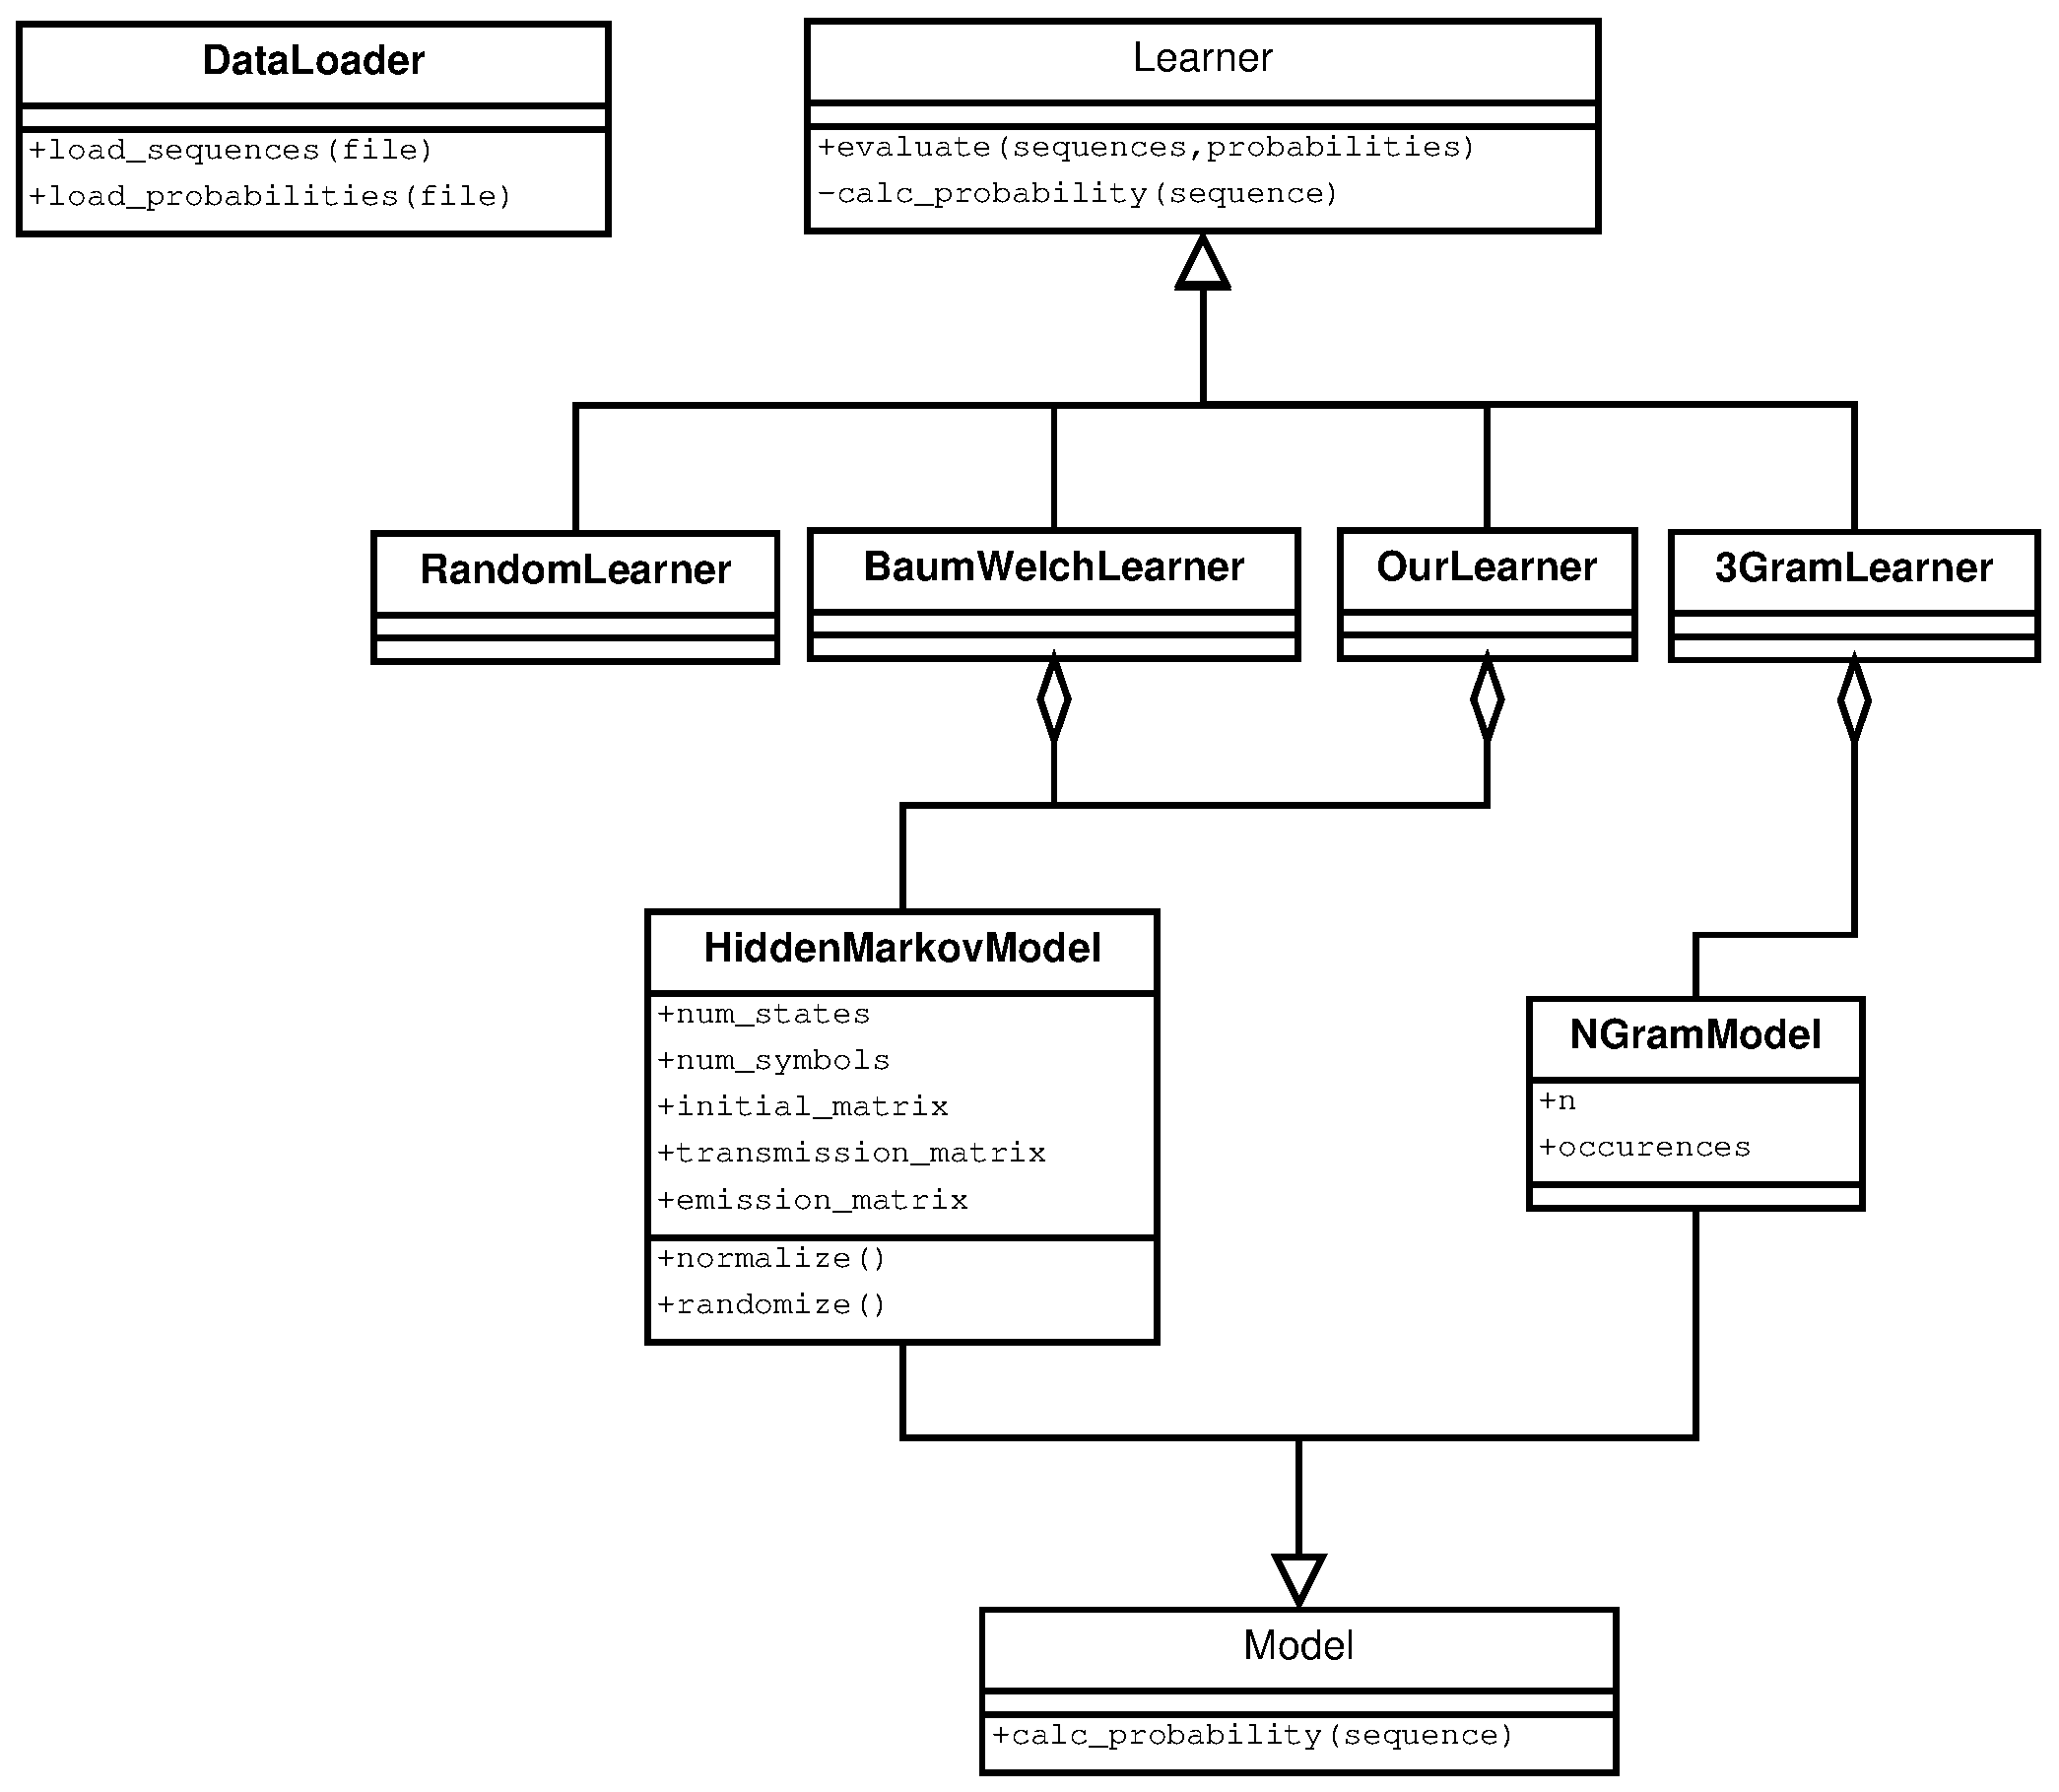
\includegraphics[scale=.4]{pictures/test-environment-overview.eps}
\caption{An overview of the test environment architecture.}
\label{fig:testenvironment}
\end{figure}
\todo{update diagram to reflect the newest version}

\subsection{Benchmark}
The \formatclass{Benchmark} class is the core element of the test environment as it is responsible for executing and tracking the actual tests and recording the results. The \formatclass{Benchmark} class is first initialised by specifying the parameters for the tests to be run and subsequently, the initialised tests are executed by calling the \formatfunction{Run()} method.

Numerous test parameters can be specified for the Benchmark, namely:

\begin{itemize}
	\item[] Data -- allows for the specification of PautomaC data files the tests are to be conducted on. The \formatclass{Benchmark} class prepares all the data in advance and uses them with the same settings for every different learner or configuration.
	\item[] Learners -- specifies which learning algorithms to test. Every chosen learner then undergoes an individual configuration to allow testing the learner in multiple different configurations.
	\item[] Number of runs -- as self-explanatory as it seems this parameter regulates the number of runs to be conducted in order to reduce possible noise.
	\item[] Training and validation set size -- regulation of how many sequences from the PautomaC train data file are to be actually used for training and validation.
	\item[] Evaluation method -- allows a choice between evaluating simply as logarithmic likelihood of the validation sequences or using the PautomaC evaluation criterion with the use of the solution data.
\end{itemize}

The \formatclass{Benchmark} class provides information through several output channels. First it sends the information on currently conducted test to the command line making it easy to determine the progress of the whole benchmarking performed. Second it provides results in two different formats at once -- a plaintext with formatting that ensures easy readability by humans and \gls{csv} to allow easy modification by other applications or loading the data into a spreadsheet editor for further analysis. All the results are updated in real time so that if the benchmark fails to finish successfully or is user interrupted in the middle at least partial results from the already finished experiments are available.

Multiple results are produced by the \formatclass{Benchmark}. Most naturally results of both the score and running time are recorded for each run, learner and configuration tested. Next a summary is added for each learner to show average and median performance over the different runs for each configuration and the best performing configuration is highlighted. A global summary through all the learners is also offered comparing their best configurations. Last but not least the learned model is saved for every run, learner and configuration so a review is possible if the results seem unnatural.

\subsection{Data}
The \formatclass{DataLoader} class is responsible for loading training data, test data and solution data from the files published at the Pautomac website. Both training and test data are expected to contain a list of sequences, while solution data is expected to contain a list of probabilities for the test sequences in accordance to the data format utilised by the PautomaC \todo{insert secref}.

The data loader stores the loaded data in an entity class called \formatclass{DataSet} passed to the \formatclass{Benchmark}. The \formatclass{DataSet} is responsible for splitting the loaded training data obtained from PautomaC data files into data to be used for the actual training and data or validation. The split is done in a pseudo-random fashion in order to ensure that multiple algorithms in different configurations will be tested on the same training and validation data, but also provide diversity through increased number of runs, where a different split is generated for each run.

As aforementioned the test environment also allows for specification of a given number of sequences to use as training or validation data. It thus becomes possible to run tests on smaller training sets in case only fast, approximate result is required.

\subsection{Evaluator}
The \formatclass{Evaluator} class is responsible for computing the score of a learner by either of the two offered evaluation criteria. As mentioned above the criteria are either the PautomaC evaluation criterion \todo{insert secref} comparing the learner directly to the solution file, or by logarithmic likelihood, which is simply a sum of logarithms of probabilities of all validation sequences given the model.

\subsection{Learner}
An integral part of the test environment is the abstract class \formatclass{Learner}. The \formatclass{Learner} provides a common interface for every implemented learning algorithm allowing the \formatclass{Benchmark} and \formatclass{Evaluator} to work with every learning approach indifferently.

The \formatclass{Learner} class specifies several methods that are implemented by individual learning algorithms and are subsequently called by either the \formatclass{Benchmark} class directly or by \formatclass{Evaluator} class:

\begin{itemize}
	\item[] \formatfunction{Initialise(learnerParameters)} -- initialises the \formatclass{Learner} into a given configuration. As different learning algorithms require different parameters a special class \formatclass{LearnerParameters} has been created to encompass all the different configuration parameters as specified by user. The \formatclass{Learner} can than obtain the relevant parameters to use them for initialisation.
	\item[] \formatfunction{CalculateProbability(sequence, logarithm)} -- Computes the probability of the specified observable state sequence given the learned model. The probability can either be returned as is or as logarithm of the probability controlled by the boolean \formatfunction{logarithm} parameter.
	\item[] \formatfunction{Learn(trainingData, validationData)} -- learns the actual model from the given training sequences. The validation sequences may and may not be used depending on the learning algorithm.
	\item[] \formatfunction{Save(outputStream, csvStream)} -- saves the learned model into two files, plaintext for readability by humans and \gls{csv} for computer manipulation.
\end{itemize}

\subsection{Models}

Our experimental algorithms ustilise the \acrlong{hmm} and only modify the learning of the model, generally still using the well known \gls{baum-welch}. To be able to provide access to commonly used algorithms such as the \gls{baum-welch} or \gls{viterbi} for every of the learning algorithms, an \gls{hmm} model class has been introduced into the test environment. The model was later implemented in three different version, as a standard \gls{hmm}, an \gls{hmm} optimised for sparse matrix (\emph{Sparse Hidden Markov Model}) and in form of a graph to allow simple structural modifications of the model. All three model versions are compatible and are directly convertible form one to another.

\subsubsection{Standard Hidden Markov Model}

The first utilised model was a standard implementation of an \gls{hmm} including the \gls{fb_algorithm}, \gls{viterbi} and \gls{baum-welch}. The original code was adopted from a tutorial by de Souza~\cite{desouza_hmm}, developer of the Accord.NET machine learning framework~\cite{accord_net}.

Several changes had to be done to the algorithms to best suit our needs. First was a memory optimisation. The algorithm was written in a way that stored the $\xi_t(i,j)$ variables as defined in section \ref{sec:baum-welch} for every of the training sequences. With up to $100000$ sequences per data file even if we were to only use half of them for training and each of them was only $8$ symbols long in average, we would need at least $32$ GB of memory to store all the $\xi_t(i,j)$ variables for a $100$ state model. A slight modification was therefore made to only store $\xi_t(i,j)$ variables for one sequence at a time achieving huge drops in memory usage.

Another change was made to modify the \gls{baum-welch} to run with different data for training and validation as the original algorithm used the same sequence set for both approximation of the parameters and subsequently to compute the logarithmic likelihood of all the sequences used to determine convergence. The new version of the algorithm works with separate training sequences for the learning itself and validation sequences for log likelihood computations.

\subsubsection{Sparse Hidden Markov Model}
\label{sec:'shmm}

As many of implemented experimental algorithms work with \glspl{hmm} that have sparse transition matrix in the sense of many transition probabilities being zero, we deemed it useful to optimise the algorithms for sparse matrix environment. For this purpose a new model, the \emph{Sparse hidden Markov model}, was implemented to utilise the sparseness of the matrix to achieve increased performance speed compared to standard methods.

The \emph{Sparse hidden Markov model} optimisation is done mainly in the form of storing information on active (non-zero probability) transitions in the model. To achieve this every node remembers all active successors and all active predecessors. This allows the algorithms to only read and compute the values relevant to the underlying \gls{hmm}, thus achieving computational speedup without loss of precision.

The above optimisation build on the property of the \gls{baum-welch} that the probability of a transition will stay as either zero or non-zero (unless an underflow occurs) during iterative update of the parameters.

The above information is utilised by both \gls{baum-welch} and \gls{fb_algorithm}, which is required for evaluation of the model and in the \gls{baum-welch} itself. The \gls{viterbi} was also optimised using the above knowledge. Exhaustive testing has been done to ensure correctness of the algorithm as well as measure the obtained speedup. The tests were conducted using randomly generated dummy data and randomly initialised models. Eight different runs were conducted for every configuration to filter out possible noise. For each run a different random initial configuration was generated and used for both the standard \gls{hmm} and the optimised sparse version. For tests of the \gls{baum-welch} $20$ iterations were conducted for each run for both the standard and sparse versions. The average speedup achieved on either the \gls{baum-welch} or \gls{viterbi} can be seen in graphs \ref{sparseBWspeedup} and \ref{sparseViterbispeedup} respectively.

\begin{figure}
	\centering
	\begin{tikzpicture}
		\begin{axis}[
			width=0.8\textwidth,
			height=0.32\textheight,
			ymin=1,
			ymax=5,
			xlabel = Number of states,
            		ylabel = Average speedup,
            		legend style={at={(0,1)}, anchor=north west}]
			\addplot+table[x=States, y=BW_8, col sep=tab]
			{content/Experiments/graphdata/sparseHMMspeedup10.csv};
			\addlegendentry{A}
			\addplot+table[x=States, y=BW_2, col sep=tab]
			{content/Experiments/graphdata/sparseHMMspeedup10.csv};
			\addlegendentry{B}
			\addplot+table[x=States, y=BW_2, col sep=tab]
			{content/Experiments/graphdata/sparseHMMspeedup5.csv};
			\addlegendentry{C}
		\end{axis}
	\end{tikzpicture}
	\caption{Average speedup achieved on \gls{baum-welch} using the \emph{Sparse hidden Markov model}. \textbf{A:} Tested a model with transition density of 10\% on dummy data with 8 symbols. \textbf{B:} Tested a model with transition density of 10\% on dummy data with 2 symbols. \textbf{C:} Tested a model with transition density of 5\% on dummy data with 2 symbols.}
	\label{sparseBWspeedup}
\end{figure}

\begin{figure}
	\centering
	\begin{tikzpicture}
		\begin{axis}[
			width=0.8\textwidth,
			height=0.32\textheight,
			ymin=10,
			ymax=40,
			xlabel = Number of states,
            		ylabel = Average speedup,
            		legend style={at={(0,1)}, anchor=north west}]
			\addplot+table[x=States, y=VIT_8, col sep=tab]
			{content/Experiments/graphdata/sparseHMMspeedup10.csv};
			\addlegendentry{A}
			\addplot+table[x=States, y=VIT_2, col sep=tab]
			{content/Experiments/graphdata/sparseHMMspeedup10.csv};
			\addlegendentry{B}
			\addplot+table[x=States, y=VIT_2, col sep=tab]
			{content/Experiments/graphdata/sparseHMMspeedup5.csv};
			\addlegendentry{C}
		\end{axis}
	\end{tikzpicture}
	\caption{Average speedup achieved on \gls{viterbi} using the \emph{Sparse hidden Markov model}. \textbf{A:} Tested a model with transition density of 10\% on dummy signal with 8 symbols of length 10000. \textbf{B:} Tested a model with transition density of 10\% on dummy signal with 2 symbols of length 10000. \textbf{C:} Tested a model with transition density of 5\% on dummy signal with 2 symbols of length 10000.}
	\label{sparseViterbispeedup}
\end{figure}

All of the performance tests were coded in C\# programming language just as the rest of the test environment and were solely single threaded. The performance speedup was measured running on a 4-core Intel Core i7-4700MQ processor machine clocked at frequency 2.4 GHz with 8 GB of available \gls{ram} and utilising the Microsoft Windows 8 operating system.

The result graph \ref{sparseBWspeedup} shows that the \gls{baum-welch} speedup using the \emph{Sparse Hidden Markov Model} is largely independent of the number of symbols in the data, however strongly correlated to the negative density (or ``sparsity'') of the model of the transition matrix. The speedup measured for the \gls{baum-welch} achieved a factor of $2.53$ for the 10\%  data density and a factor of $4.72$ for the 5\% density for a $100$ state model. The observed speedup is lower than the expected theoretical value (factor of 10 for 10\% density and 20 for 5\% density). This may be caused by unideal implementation, use of more and more complex data structures and possibly optimisation performed by the compiler.

A significant speedup has been observed for the \gls{viterbi}. As can be observed from the result graph, \ref{sparseViterbispeedup}, the speedup on the \gls{viterbi} is very similar to speedup on \gls{baum-welch}, being independent on the number of symbols and almost linear to sparsity of the model. A speedup by a factor of $20.99$ has been observed for the model with 10\% density, but this factor was increased to $38.01$ with 5\% density model. Both of the discussed results are the highest measured speedups observed for $100$ state models. Contrary to \gls{baum-welch} results, \gls{viterbi} scored better than the expected theoretical speedup.

\subsubsection{HMM Graph}

\section{Selecting Datasets}\label{sec:datasets}
In the Pautomac competition, 48 data sets were used. If we were to conduct experiments on all of those data sets, it would take an unreasonable amount of time.
As a consequence, we have chosen to limit the amount of data sets used in our experiments.
We think the most important parameters that differs between data sets are the number of states used by the generating model, the number of symbols, and the transition density. The number of states and symbols have been published after the competition finished, and the transition density is something we can calculate by examining the models that generated each data set, which was also published when the competition finished.
We define the transition density as the ratio between the number of transitions in the model and the number of states squared (the total number of possible transitions). 

For each of the 3 parameters, 4 data sets have been selected that differ as much as possible on that particular parameter, while the other two parameters differ as little as possible.
Figure \ref{fig:statesetplot} shows how four data sets represent different amount of states, while the number of symbols and transition density almost stay the same. In \ref{density_table} and \ref{symbol_table}, a smilar scatterplot can be seen for the transition density and the number of symbols, respectively.

\begin{figure}
	\centering
	\begin{subfigure}[b]{0.5\textwidth}
        	\begin{tikzpicture}
			\begin{axis}[
			scale = 0.8,
			xlabel = Transition density (\%),
            	ylabel = Number of symbols]
			\addplot[scatter,
				only marks,
				scatter src=explicit] 
				table[meta=mark, x=density, y=symbols, col sep=tab]
				{content/Experiments/graphdata/stateset.csv};
			\end{axis}
		\end{tikzpicture}
        \end{subfigure}%
		\begin{subfigure}[b]{0.5\textwidth}
\begin{tikzpicture}
	\begin{axis}[
	scale = 0.8,
			xlabel = Number of states,
            	ylabel = Number of symbols]
		\addplot[scatter,
			only marks,
			scatter src=explicit] 
		table[meta=mark, x=states, y=symbols, col sep=tab]
		{content/Experiments/graphdata/stateset.csv};
	\end{axis}
\end{tikzpicture}
	\end{subfigure}
  	\caption{Two plots visualising the selected state-range datasets}\label{fig:statesetplot}
\end{figure}

%%%%%%%%%%%%%%%%%%%%%%%
%
%_______density range______________

\begin{figure}
	\centering
	\begin{subfigure}[b]{0.5\textwidth}
        	\begin{tikzpicture}
			\begin{axis}[
			scale = 0.8,
			xlabel = Number of states,
            	ylabel = Number of symbols]
			\addplot[scatter,
				only marks,
				scatter src=explicit] 
				table[meta=mark, x=states, y=symbols, col sep=tab]
				{content/Experiments/graphdata/densityset.csv};
			\end{axis}
		\end{tikzpicture}
		\end{subfigure}%
		\begin{subfigure}[b]{0.5\textwidth}
		\begin{tikzpicture}
	\begin{axis}[
			scale = 0.8,
			xlabel = Transition density(\%),
            	ylabel = Number of symbols]
		\addplot[scatter,
			only marks,
			scatter src=explicit] 
		table[meta=mark, x=density, y=symbols, col sep=tab]
		{content/Experiments/graphdata/densityset.csv};
	\end{axis}
\end{tikzpicture}
\end{subfigure}
  	\caption{Two plots visualising the selected density-range datasets}\label{fig:densitysetplot}
\end{figure}

%%%%%%%%%%%%%%%%%%%%%%%
%
%_______symbol range______________

\begin{figure}
	\centering
	\begin{subfigure}[b]{0.5\textwidth}
        	\begin{tikzpicture}
			\begin{axis}[
			scale = 0.8,
			xlabel = Transition density(\%),
            	ylabel = Number of states]
			\addplot[scatter,
				only marks,
				scatter src=explicit] 
				table[meta=mark, x=density, y=states, col sep=tab]
				{content/Experiments/graphdata/symbolset.csv};
			\end{axis}
		\end{tikzpicture}
       \end{subfigure}%
	\begin{subfigure}[b]{0.5\textwidth}
		\begin{tikzpicture}
			\begin{axis}[
			scale = 0.8,
			xlabel = Number of symbols,
            	ylabel = Number of states]
		\addplot[scatter,
			only marks,
			scatter src=explicit] 
		table[meta=mark, x=symbols, y=states, col sep=tab]
		{content/Experiments/graphdata/symbolset.csv};
	\end{axis}
	\end{tikzpicture}
	\end{subfigure}
  	\caption{Two plots visualising the selected symbol-range datasets}\label{fig:symbolsetplot}
\end{figure}

\FloatBarrier

\begin{table}
\centering
{
\begin{tabular}{| c | c | c | c |}
  \hline
  Dataset 	& \textbf{States} 	& Density (\%) 	& Symbols \\  \hline
  6 			& \textbf{19 }			&	13.5				& 6 \\
  23 			& \textbf{33} 			&	11.4				& 7 \\
  41			& \textbf{54} 			&	14.3				& 7 \\
  1				& \textbf{64} 			&	8.7				& 8 \\ \hline
\end{tabular}
\caption{State amount}
\label{state_table}
}
\end{table}

\begin{table}
\centering
{
\begin{tabular}{| c | c | c | c |}
  \hline
  Dataset 	& States  			& \textbf{Density (\%)} 		& Symbols \\  \hline
  36 			&	54					& \textbf{7.4 }						& 9 \\
  8 			&	49					& \textbf{16.8 }					& 7 \\
  43			&	67					& \textbf{40.2 }					& 5 \\
  37			&	69					& \textbf{54 	}					& 8 \\ \hline
\end{tabular}
\caption{Transition density percentage}
\label{density_table}
}
\end{table}

\begin{table}
\centering
{
\begin{tabular}{| c | c | c | c |}
  \hline
  Dataset 	& States	 	& Density (\%) 	& \textbf{Symbols}	 \\  \hline
  32 			& 43				& 11.8				& \textbf{4}		\\
  8 			& 49				& 16.7 				& \textbf{8}		\\
  10			& 49				& 14.2 				& \textbf{11}	\\
  35			& 47				& 14.2 				& \textbf{20}	\\ \hline
\end{tabular}
\caption{Symbol alphabet size}
\label{symbol_table}

}
\end{table}
\section{Selecting Algorithm Parameters}
5000 sequences train/validate
10 - 100 states
10 step

\subsection{Baum-Welch Treshold}
Baum-Welch takes 

\begin{figure}
	\begin{tikzpicture}
		\begin{axis}[
				ybar,
				xtick=data,
   				symbolic x coords={0.1,0.05,0.01,0.005,0.001,0.0001},
				xlabel = Treshold,
            		ylabel = Score (lower is better)]
				\addplot+table[y=Score, col sep=tab]
				{content/Experiments/treshold.csv};
		\end{axis}
	\end{tikzpicture} 
\caption{Loglikelyhood when running Baum-Welch with a treshold}
\label{fig:treshold}
\end{figure}

\subsection{Greedy Extend}
10 BW iterations
100 attempts
\FloatBarrier

\section{Dataset experiments}
The approach used for each dataset parameter experiment have been to cover a range of state amounts, ranging from 10 to 100 states, together with the previously define parameters. \gls{bw} was probed on specific state amounts with step sizes of 10, where the dynamic algorithms have been defined to reach either some local maxima or stop at 100 states.

\subsection{State Space Experiments}

The purpose of the state experiments are to show how \gls{bw} and our own algorithms and models perform in relation to different number of states.\\

	\begin{figure}[h]
\begin{tabular*}{\textwidth}{@{}cc@{}}
\begin{minipage}{\dimexpr0.55\textwidth-2\tabcolsep}
\centering
\textbf{Data set: 6, States: 19}\par\medskip
\begin{tikzpicture}
	\pgfplotsset{every axis legend/.append style={ 
		at={(0.5,1.1)},
		anchor=south}}
	\begin{axis}[
			scaled ticks = true,
			scaled y ticks=base 10:-4,
			xlabel = Number of states,
            	ylabel = Log likelihood,
            	legend columns=-1,
            	legend entries={BW, SBW, GE, GS},
			legend style={/tikz/every even column/.append style={column sep=0.3cm}}]
			
		\addplot+table[x=States, y=BW, col sep=tab]
		{content/Experiments/graphdata/set6.csv};
%		\addlegendentry{\textbf{BW}}
		
		\addplot+table[x=States, y=SBW, col sep=tab]
		{content/Experiments/graphdata/set6.csv};
%		\addlegendentry{\textbf{Sparse BW}}
		
		\addplot+table[x=States, y=GE, col sep=tab]
		{content/Experiments/graphdata/set6.csv};
		
		\addplot+table[x=States, y=Padawan, col sep=tab]
		{content/Experiments/graphdata/set6.csv};
%		\addlegendentry{\textbf{Greedy Extend}}
	\end{axis}
\end{tikzpicture} 
\end{minipage}% 
&
\begin{minipage}{\dimexpr0.55\textwidth-2\tabcolsep}
\centering
\textbf{Data set: 23, States: 33}\par\medskip
\begin{tikzpicture}
	\pgfplotsset{every axis legend/.append style={ 
		at={(0.5,1.1)},
		anchor=south}}
	\begin{axis}[
			scaled ticks = true,
			scaled y ticks=base 10:-4,
			xlabel = Number of states,
            	ylabel = Score (lower is better),
            	legend columns=-1,
            	legend entries={BW, SBW, GE, GS},
			legend style={/tikz/every even column/.append style={column sep=0.3cm}}]
			
		\addplot+table[x=States, y=BW, col sep=tab]
		{content/Experiments/graphdata/set23.csv};
%		\addlegendentry{\textbf{BW}}
		
		\addplot+table[x=States, y=SBW, col sep=tab]
		{content/Experiments/graphdata/set23.csv};
%		\addlegendentry{\textbf{Sparse BW}}
		
		\addplot+table[x=States, y=GE, col sep=tab]
		{content/Experiments/graphdata/set23.csv};
		
		\addplot+table[x=States, y=Padawan, col sep=tab]
		{content/Experiments/graphdata/set23.csv};
%		\addlegendentry{\textbf{Greedy Extend}}
	\end{axis}
\end{tikzpicture} 
\end{minipage}
\\
\begin{minipage}[t]{\dimexpr0.6\textwidth-2\tabcolsep}
\end{minipage}
&
\begin{minipage}[t]{\dimexpr0.4\textwidth-2\tabcolsep}
\end{minipage}
\end{tabular*}%
\\
\begin{tabular*}{\textwidth}{@{}cc@{}}
\begin{minipage}{\dimexpr0.55\textwidth-2\tabcolsep}
\centering
\textbf{Data set: 41, States: 54}\par\medskip
\begin{tikzpicture}
	\pgfplotsset{every axis legend/.append style={ 
		at={(0.5,1.1)},
		anchor=south}}
	\begin{axis}[
			scaled ticks = true,
			scaled y ticks=base 10:-4,
			xlabel = Number of states,
            	ylabel = Score (lower is better),
            	legend columns=-1,
            	legend entries={BW, SBW, GE, GS},
			legend style={/tikz/every even column/.append style={column sep=0.3cm}}]
			
		\addplot+table[x=States, y=BW, col sep=tab]
		{content/Experiments/graphdata/set41.csv};
%		\addlegendentry{\textbf{BW}}
		
		\addplot+table[x=States, y=SBW, col sep=tab]
		{content/Experiments/graphdata/set41.csv};
%		\addlegendentry{\textbf{Sparse BW}}
		
		\addplot+table[x=States, y=GE, col sep=tab]
		{content/Experiments/graphdata/set41.csv};
		
		\addplot+table[x=States, y=Padawan, col sep=tab]
		{content/Experiments/graphdata/set41.csv};
%		\addlegendentry{\textbf{Greedy Extend}}
	\end{axis}
\end{tikzpicture} 
\end{minipage}% 
&
\begin{minipage}{\dimexpr0.55\textwidth-2\tabcolsep}
\centering
\textbf{Data set: 1, States: 64}\par\medskip
\begin{tikzpicture}
	\pgfplotsset{every axis legend/.append style={ 
		at={(0.5,1.1)},
		anchor=south}}
	\begin{axis}[
			scaled ticks = true,
			scaled y ticks=base 10:-4,
			xlabel = Number of states,
            	ylabel = Log likelihood,
            	legend columns=-1,
            	legend entries={BW, SBW, GE, GS},
			legend style={/tikz/every even column/.append style={column sep=0.3cm}}]
			
		\addplot+table[x=States, y=BW, col sep=tab]
		{content/Experiments/graphdata/set1.csv};
%		\addlegendentry{\textbf{BW}}
		
		\addplot+table[x=States, y=SBW, col sep=tab]
		{content/Experiments/graphdata/set1.csv};
%		\addlegendentry{\textbf{Sparse BW}}
		
		\addplot+table[x=States, y=GE, col sep=tab]
		{content/Experiments/graphdata/set1.csv};
		
		\addplot+table[x=States, y=Padawan, col sep=tab]
		{content/Experiments/graphdata/set1.csv};
%		\addlegendentry{\textbf{Greedy Extend}}
	\end{axis}
\end{tikzpicture} 
\end{minipage}
\\
\begin{minipage}[t]{\dimexpr0.6\textwidth-2\tabcolsep}
\end{minipage}
\end{tabular*}%
\caption{Four data sets produced by models with 19 to 64 states}\label{fig:states}
\end{figure}

In Figure \ref{fig:states} the ranges of log likelihood should be noted carefully. A large likelihood difference exist between the data sets, which can at least partly be explained by the observed sequences in the data sets. A higher complexity of the data sequences will naturally be harder to learn. For instance data set 41 seems to have a lower likelihood than data set 6. Looking into the sequences of these two data sets we find that data set 41 has an average sequence length of 7,3 characters, using 7 different symbols, whereas data set 6 has an average sequence length of 14,7 characters, using 6 different symbols. From these numbers it is clear that the amount of possible combinations is much lower for data set 41, compared to data set 6.




Initial observations
\begin{itemize}
\item GE performs the best, except dataset 1. It seems like GE would surpass BW with a larger state space.
\item SBW performs worse than BW, note that dataset 41 has a fairly small y-axis, where the best GE result is about 800 points. We estimate an error margin of 100-200 points. Without more runs for each experiment, it is impossible to determine an exact error margin.
\item In general we seem to 
\end{itemize}


\subsection{Transition Density Experiments}

The purpose of the transition density experiments are to show how \gls{bw} and our own algorithms and models perform in relation to the transition density.\\

	\FloatBarrier
\section{Results}
\subsection{State Experiments}

\begin{tabular*}{\textwidth}{@{}cc@{}}
\begin{minipage}{\dimexpr0.55\textwidth-2\tabcolsep}
\centering
\textbf{Dataset: 6, States: 19}\par\medskip
\begin{tikzpicture}
	\begin{axis}[
			xlabel = Number of states,
            	ylabel = Score (lower is better)]
		\addplot+table[x=States, y=BW, col sep=tab]
		{content/Experiments/graphdata/set6.csv};
		\addlegendentry{\textbf{BW}}
		
		\addplot+table[x=States, y=SBW, col sep=tab]
		{content/Experiments/graphdata/set6.csv};
		\addlegendentry{\textbf{Sparse BW}}
		
		\addplot+table[x=States, y=GE, col sep=tab]
		{content/Experiments/graphdata/set6.csv};
		\addlegendentry{\textbf{Greedy Extend}}
	\end{axis}
\end{tikzpicture} 
\label{fig:dataset6}
\end{minipage}% 
&
\begin{minipage}{\dimexpr0.55\textwidth-2\tabcolsep}
\centering
\textbf{Dataset: 23, States: 33}\par\medskip
\begin{tikzpicture}
	\begin{axis}[
			xlabel = Number of states,
            	ylabel = Score (lower is better)]
		\addplot+table[x=States, y=BW, col sep=tab]
		{content/Experiments/graphdata/set23.csv};
		\addlegendentry{\textbf{BW}}
		
		\addplot+table[x=States, y=SBW, col sep=tab]
		{content/Experiments/graphdata/set23.csv};
		\addlegendentry{\textbf{Sparse BW}}
		
		\addplot+table[x=States, y=GE, col sep=tab]
		{content/Experiments/graphdata/set23.csv};
		\addlegendentry{\textbf{Greedy Extend}}
	\end{axis}
\end{tikzpicture} 
\label{fig:dataset23}
\end{minipage}
\\
\begin{minipage}[t]{\dimexpr0.6\textwidth-2\tabcolsep}
\end{minipage}
&
\begin{minipage}[t]{\dimexpr0.4\textwidth-2\tabcolsep}
\end{minipage}
\end{tabular*}%


begin{tabular*}{\textwidth}{@{}cc@{}}
\begin{minipage}{\dimexpr0.55\textwidth-2\tabcolsep}
\centering
\textbf{Dataset: 41, States: 54}\par\medskip
\begin{tikzpicture}
	\begin{axis}[
			xlabel = Number of states,
            	ylabel = Score (lower is better)]
		\addplot+table[x=States, y=BW, col sep=tab]
		{content/Experiments/graphdata/set41.csv};
		\addlegendentry{\textbf{BW}}
		
		\addplot+table[x=States, y=SBW, col sep=tab]
		{content/Experiments/graphdata/set41.csv};
		\addlegendentry{\textbf{Sparse BW}}
		
		\addplot+table[x=States, y=GE, col sep=tab]
		{content/Experiments/graphdata/set41.csv};
		\addlegendentry{\textbf{Greedy Extend}}
	\end{axis}
\end{tikzpicture} 
\label{fig:dataset41}
\end{minipage}% 
&
\begin{minipage}{\dimexpr0.55\textwidth-2\tabcolsep}
\centering
\textbf{Dataset: 1, States: 64}\par\medskip
\begin{tikzpicture}
	\begin{axis}[
			xlabel = Number of states,
            	ylabel = Score (lower is better)]
		\addplot+table[x=States, y=BW, col sep=tab]
		{content/Experiments/graphdata/set64.csv};
		\addlegendentry{\textbf{BW}}
		
		\addplot+table[x=States, y=SBW, col sep=tab]
		{content/Experiments/graphdata/set64.csv};
		\addlegendentry{\textbf{Sparse BW}}
		
		\addplot+table[x=States, y=GE, col sep=tab]
		{content/Experiments/graphdata/set64.csv};
		\addlegendentry{\textbf{Greedy Extend}}
	\end{axis}
\end{tikzpicture} 
\label{fig:dataset64}
\end{minipage}
\\
\begin{minipage}[t]{\dimexpr0.6\textwidth-2\tabcolsep}
\end{minipage}
&
\begin{minipage}[t]{\dimexpr0.4\textwidth-2\tabcolsep}
\end{minipage}
\end{tabular*}%

\subsection{Density Experiments}

\FloatBarrier
\begin{tabular*}{\textwidth}{@{}cc@{}}
\begin{minipage}{\dimexpr0.55\textwidth-2\tabcolsep}
\centering
\begin{tikzpicture}
	\begin{axis}[
			xlabel = Number of states,
            	ylabel = Score (lower is better)]
		\addplot+table[x=States, y=BW, col sep=tab]
		{content/Experiments/graphdata/set23.csv};
		\addlegendentry{\textbf{BW}}
		
		\addplot+table[x=States, y=SBW, col sep=tab]
		{content/Experiments/graphdata/set23.csv};
		\addlegendentry{\textbf{Sparse BW}}
		
		\addplot+table[x=States, y=GE, col sep=tab]
		{content/Experiments/graphdata/set23.csv};
		\addlegendentry{\textbf{Greedy Extend}}
		
	\end{axis}
\end{tikzpicture}
\label{dataset23}
\end{minipage}% 
&
\begin{minipage}{\dimexpr0.55\textwidth-2\tabcolsep}
\centering
\begin{tikzpicture}
	\begin{axis}[
			xlabel = Number of states,
            	ylabel = Score (lower is better)]
		\addplot+table[x=States, y=BW, col sep=tab]
		{content/Experiments/graphdata/set1.csv};
		\addlegendentry{\textbf{Dataset: 1 States: 64}}
	\end{axis}
\end{tikzpicture}
\label{dataset1}
\end{minipage}
\\
\begin{minipage}[t]{\dimexpr0.6\textwidth-2\tabcolsep}
\end{minipage}
&
\begin{minipage}[t]{\dimexpr0.4\textwidth-2\tabcolsep}
\end{minipage}
\end{tabular*}%

\begin{tabular*}{\textwidth}{@{}cc@{}}
\begin{minipage}{\dimexpr0.55\textwidth-2\tabcolsep}
\centering
\begin{tikzpicture}
	\begin{axis}[
			xlabel = Number of states,
            	ylabel = Score (lower is better)]
		\addplot+table[x=States, y=BW, col sep=tab]
		{content/Experiments/graphdata/set23.csv};
		\addlegendentry{\textbf{Dataset: 23 States: 33}}
	\end{axis}
\end{tikzpicture}
\label{dataset23}
\end{minipage}% 
&
\begin{minipage}{\dimexpr0.55\textwidth-2\tabcolsep}
\centering
\begin{tikzpicture}
	\begin{axis}[
			xlabel = Number of states,
            	ylabel = Score (lower is better)]
		\addplot+table[x=States, y=BW, col sep=tab]
		{content/Experiments/graphdata/set1.csv};
		\addlegendentry{\textbf{Dataset: 1 States: 64}}
	\end{axis}
\end{tikzpicture}
\label{dataset1}
\end{minipage}
\\
\begin{minipage}[t]{\dimexpr0.6\textwidth-2\tabcolsep}
\end{minipage}
&
\begin{minipage}[t]{\dimexpr0.4\textwidth-2\tabcolsep}
\end{minipage}
\end{tabular*}%

\subsection{Symbol size Experiments}

\begin{tabular*}{\textwidth}{@{}cc@{}}
\begin{minipage}{\dimexpr0.55\textwidth-2\tabcolsep}
\centering
\textbf{Dataset: 6, States: 19}\par\medskip
\begin{tikzpicture}
	\begin{axis}[
			xlabel = Number of states,
            	ylabel = Score (lower is better)]
		\addplot+table[x=States, y=BW, col sep=tab]
		{content/Experiments/graphdata/set6.csv};
		\addlegendentry{\textbf{BW}}
		
		\addplot+table[x=States, y=SBW, col sep=tab]
		{content/Experiments/graphdata/set6.csv};
		\addlegendentry{\textbf{Sparse BW}}
		
		\addplot+table[x=States, y=GE, col sep=tab]
		{content/Experiments/graphdata/set6.csv};
		\addlegendentry{\textbf{Greedy Extend}}
	\end{axis}
\end{tikzpicture} 
\label{fig:dataset6}
\end{minipage}% 
&
\begin{minipage}{\dimexpr0.55\textwidth-2\tabcolsep}
\centering
\textbf{Dataset: 23, States: 33}\par\medskip
\begin{tikzpicture}
	\begin{axis}[
			xlabel = Number of states,
            	ylabel = Score (lower is better)]
		\addplot+table[x=States, y=BW, col sep=tab]
		{content/Experiments/graphdata/set23.csv};
		\addlegendentry{\textbf{BW}}
		
		\addplot+table[x=States, y=SBW, col sep=tab]
		{content/Experiments/graphdata/set23.csv};
		\addlegendentry{\textbf{Sparse BW}}
		
		\addplot+table[x=States, y=GE, col sep=tab]
		{content/Experiments/graphdata/set23.csv};
		\addlegendentry{\textbf{Greedy Extend}}
	\end{axis}
\end{tikzpicture} 
\label{fig:dataset23}
\end{minipage}
\\
\begin{minipage}[t]{\dimexpr0.6\textwidth-2\tabcolsep}
\end{minipage}
&
\begin{minipage}[t]{\dimexpr0.4\textwidth-2\tabcolsep}
\end{minipage}
\end{tabular*}%


begin{tabular*}{\textwidth}{@{}cc@{}}
\begin{minipage}{\dimexpr0.55\textwidth-2\tabcolsep}
\centering
\textbf{Dataset: 41, States: 54}\par\medskip
\begin{tikzpicture}
	\begin{axis}[
			xlabel = Number of states,
            	ylabel = Score (lower is better)]
		\addplot+table[x=States, y=BW, col sep=tab]
		{content/Experiments/graphdata/set41.csv};
		\addlegendentry{\textbf{BW}}
		
		\addplot+table[x=States, y=SBW, col sep=tab]
		{content/Experiments/graphdata/set41.csv};
		\addlegendentry{\textbf{Sparse BW}}
		
		\addplot+table[x=States, y=GE, col sep=tab]
		{content/Experiments/graphdata/set41.csv};
		\addlegendentry{\textbf{Greedy Extend}}
	\end{axis}
\end{tikzpicture} 
\label{fig:dataset41}
\end{minipage}% 
&
\begin{minipage}{\dimexpr0.55\textwidth-2\tabcolsep}
\centering
\textbf{Dataset: 1, States: 64}\par\medskip
\begin{tikzpicture}
	\begin{axis}[
			xlabel = Number of states,
            	ylabel = Score (lower is better)]
		\addplot+table[x=States, y=BW, col sep=tab]
		{content/Experiments/graphdata/set64.csv};
		\addlegendentry{\textbf{BW}}
		
		\addplot+table[x=States, y=SBW, col sep=tab]
		{content/Experiments/graphdata/set64.csv};
		\addlegendentry{\textbf{Sparse BW}}
		
		\addplot+table[x=States, y=GE, col sep=tab]
		{content/Experiments/graphdata/set64.csv};
		\addlegendentry{\textbf{Greedy Extend}}
	\end{axis}
\end{tikzpicture} 
\label{fig:dataset64}
\end{minipage}
\\
\begin{minipage}[t]{\dimexpr0.6\textwidth-2\tabcolsep}
\end{minipage}
&
\begin{minipage}[t]{\dimexpr0.4\textwidth-2\tabcolsep}
\end{minipage}
\end{tabular*}%

Initial observations
\begin{itemize}
\item GE performs the best
\item 
\item 
\end{itemize}

\subsection{Symbol Alphabet Size Experiments}
The purpose of the s are to show how \gls{bw} and our own algorithms and models perform in relation to the size of the emission symbol alphabet size.\\

	\begin{tabular*}{\textwidth}{@{}cc@{}}
\begin{minipage}{\dimexpr0.55\textwidth-2\tabcolsep}
\centering
\textbf{Dataset: 32, Symbols: 4}\par\medskip
\begin{tikzpicture}
	\pgfplotsset{every axis legend/.append style={ 
		at={(0.55,1.03)},
		anchor=south}}
	\begin{axis}[
			scaled ticks = true,
			scaled y ticks=base 10:-4,
			xlabel = Number of states,
            	ylabel = Score (lower is better),
            	legend columns=-1,
            	legend entries={BW, SBW, GE},
			legend style={/tikz/every even column/.append style={column sep=0.3cm}}]
			
		\addplot+table[x=States, y=BW, col sep=tab]
		{content/Experiments/graphdata/set32.csv};
%		\addlegendentry{\textbf{BW}}
		
		\addplot+table[x=States, y=SBW, col sep=tab]
		{content/Experiments/graphdata/set32.csv};
%		\addlegendentry{\textbf{Sparse BW}}
		
		\addplot+table[x=States, y=GE, col sep=tab]
		{content/Experiments/graphdata/set32.csv};
%		\addlegendentry{\textbf{Greedy Extend}}
	\end{axis}
\end{tikzpicture} 
\label{fig:dataset32}
\end{minipage}% 
&
\begin{minipage}{\dimexpr0.55\textwidth-2\tabcolsep}
\centering
\textbf{Dataset: 8, Symbols: 8}\par\medskip
\begin{tikzpicture}
	\pgfplotsset{every axis legend/.append style={ 
		at={(0.55,1.03)},
		anchor=south}}
	\begin{axis}[
			scaled ticks = true,
			scaled y ticks=base 10:-4,
			xlabel = Number of states,
            	ylabel = Score (lower is better),
            	legend columns=-1,
            	legend entries={BW, SBW, GE},
			legend style={/tikz/every even column/.append style={column sep=0.3cm}}]
			
		\addplot+table[x=States, y=BW, col sep=tab]
		{content/Experiments/graphdata/set8.csv};
%		\addlegendentry{\textbf{BW}}
		
		\addplot+table[x=States, y=SBW, col sep=tab]
		{content/Experiments/graphdata/set8.csv};
%		\addlegendentry{\textbf{Sparse BW}}
		
		\addplot+table[x=States, y=GE, col sep=tab]
		{content/Experiments/graphdata/set8.csv};
%		\addlegendentry{\textbf{Greedy Extend}}
	\end{axis}
\end{tikzpicture} 
\label{fig:dataset8}
\end{minipage}
\\
\begin{minipage}[t]{\dimexpr0.6\textwidth-2\tabcolsep}
\end{minipage}
&
\begin{minipage}[t]{\dimexpr0.4\textwidth-2\tabcolsep}
\end{minipage}
\end{tabular*}%
\\
\begin{tabular*}{\textwidth}{@{}cc@{}}
\begin{minipage}{\dimexpr0.55\textwidth-2\tabcolsep}
\centering
\textbf{Dataset: 10, Symbols: 11}\par\medskip
\begin{tikzpicture}
	\pgfplotsset{every axis legend/.append style={ 
		at={(0.55,1.03)},
		anchor=south}}
	\begin{axis}[
			scaled ticks = true,
			scaled y ticks=base 10:-4,
			xlabel = Number of states,
            	ylabel = Score (lower is better),
            	legend columns=-1,
            	legend entries={BW, SBW, GE},
			legend style={/tikz/every even column/.append style={column sep=0.3cm}}]
			
		\addplot+table[x=States, y=BW, col sep=tab]
		{content/Experiments/graphdata/set10.csv};
%		\addlegendentry{\textbf{BW}}
		
		\addplot+table[x=States, y=SBW, col sep=tab]
		{content/Experiments/graphdata/set10.csv};
%		\addlegendentry{\textbf{Sparse BW}}
		
		\addplot+table[x=States, y=GE, col sep=tab]
		{content/Experiments/graphdata/set10.csv};
%		\addlegendentry{\textbf{Greedy Extend}}
	\end{axis}
\end{tikzpicture} 
\label{fig:dataset41}
\end{minipage}% 
&
\begin{minipage}{\dimexpr0.55\textwidth-2\tabcolsep}
\centering
\textbf{Dataset: 35, Symbols: 20}\par\medskip
\begin{tikzpicture}
	\pgfplotsset{every axis legend/.append style={ 
		at={(0.55,1.03)},
		anchor=south}}
	\begin{axis}[
			scaled ticks = true,
			scaled y ticks=base 10:-4,
			xlabel = Number of states,
            	ylabel = Score (lower is better),
            	legend columns=-1,
            	legend entries={BW, SBW, GE},
			legend style={/tikz/every even column/.append style={column sep=0.3cm}}]
			
		\addplot+table[x=States, y=BW, col sep=tab]
		{content/Experiments/graphdata/set35.csv};
%		\addlegendentry{\textbf{BW}}
		
		\addplot+table[x=States, y=SBW, col sep=tab]
		{content/Experiments/graphdata/set35.csv};
%		\addlegendentry{\textbf{Sparse BW}}
		
		\addplot+table[x=States, y=GE, col sep=tab]
		{content/Experiments/graphdata/set35.csv};
%		\addlegendentry{\textbf{Greedy Extend}}
	\end{axis}
\end{tikzpicture}
\label{fig:dataset35}
\end{minipage}
\\
\begin{minipage}[t]{\dimexpr0.6\textwidth-2\tabcolsep}
\end{minipage}
&
\begin{minipage}[t]{\dimexpr0.4\textwidth-2\tabcolsep}
\end{minipage}
\end{tabular*}%
	
Initial observations
\begin{itemize}
\item BW performs the best on 3 out of 4 sets
\item 
\item 
\end{itemize}	
	
%\subsection{Greedy Extend Experiments}
	%\subsection{Greedy Extend}

The first big question about the Greedy Extend algorithm, is how the choice of $\beta$ affects the performance of the algorithm.
As $\beta$ denotes the iterations of Baum Welch to run each time the algorithm attempts to extend the graph, increasing $\beta$ will also increase the run time of the algorithm. It may be the case that better results are achieved when $\beta$ is increased, since more iterations of Baum Welch also means a greater increase in likelihood. However, it could be the case that using many iterations early increases the chance of getting trapped in a local optimum.
An experiment has been conducted of using different values for $\beta$ on data set $1$ from the Pautomac competition. The results can be seen in figure \ref{fig:ge-different-thresholds-tested}. Each line represents an average over 5 runs of Greedy Extend with the specified number of iterations.
  
\begin{tikzpicture}
\begin{axis}[xlabel={$x$},ylabel={Column Data}]

\addplot table[x index=0,y index=1,col sep=tab] {content/Experiments/graphdata/ge-intermediate-iterations-test.csv};
\addlegendentry{Iterations: 0}
  
\addplot table[x index=0,y index=2,col sep=tab] {content/Experiments/graphdata/ge-intermediate-iterations-test.csv};
\addlegendentry{Iterations: 1}

\end{axis}
\end{tikzpicture}  


\subsection{Speed Comparison}

Apart from scoring the individual learning algorithms by logarithmic likelihood or PautomaC evaluation criterion we have also recorded their running time. A special test was conducted to determine the performance benefits of sparsity and other approaches. The Baum-Welch Learner and Sparse Baum-Welch Learner were run for a model of size $5$ and subsequently on models $5$ hidden state larger. Both algorithms were run for exactly 8 hours to observe what results can be obtained during the given time frame. The Greedy Extend Learner was also run for 8 hours to see if the achieved growth can be faster than continuous tests on aforementioned algorithms.

The experiments were conducted using PautomaC dataset number 23. This dataset was chosen as the underlying model used by PautomaC had an average amount of states (33), rather low transition density (11.48\%) and number of symbols (7) making it considerably simple, but not too much. The experiments were run with the same parameters as the main tests, thus with convergence threshold of $0.01$, and a training and validation sets of $5000$ sequences.

The obtained results as shown in regard to score (graph \ref{fig:eight_hour_run}) and running time(graph \ref{fig:bw_vs_sbw}) are speaking in favour of the Greedy Extend Learner, whilst Sparse Baum-Welch Learner achieved the worst performance. This might be attributed to the fact that the transition matrix for the Sparse Baum-Welch Learner is randomly generated, thus even the $nlog(n)$ non-zero transitions are picked by random and the topology of the hidden state space graph cannot be considered data derived.

The tests were run on the same machine as the average speedup tests for the \hyperref[sec:shmm]{Sparse hidden Markov model} with the following configuration:
\begin{itemize}
	\item[] Intel Core i7-4700MQ processor clocked at 2.4 GHz.
	\item[] 8 GB \gls{ram}.
	\item[] Microsoft Windows 8 operating system.
\end{itemize}

\begin{figure}
	\centering
	\begin{tikzpicture}
		\begin{axis}[
			width=0.92\textwidth,
			height=0.76\textheight,
			ymax=0,
			xmin=0,
			xlabel = Number of States,
            		ylabel = Logarithmic Likelihood,
            		legend style={at={(0,1)}, anchor=north west}]
			\addplot+[mark=none]table[x=States, y=Score, col sep=tab]
			{content/Experiments/graphdata/8h_run_BW.csv};
			\addlegendentry{Baum-Welch Learner}
			\addplot+[mark=none]table[x=States, y=Score, col sep=tab]
			{content/Experiments/graphdata/8h_run_SBW.csv};
			\addlegendentry{Sparse Baum-Welch Learner}
			\addplot+[mark=none]table[x=States, y=Score, col sep=tab]
			{content/Experiments/graphdata/8h_run_GE.csv};
			\addlegendentry{Greedy Extend Learner}
		\end{axis}
	\end{tikzpicture}
	\caption{Results achieved in a time scope of eight hours.}
	\label{fig:eight_hour_run}
\end{figure}

In regards to logarithmic likelihood we may observe from the result graph \ref{fig:eight_hour_run} that both Baum-Welch and Sparse Baum-Welch Learners reach what could be called a convergence of the logarithmic likelihood score when increasing the number of states. The relatively stable value is reached at around 45 states for the Baum-Welch Learner with all the subsequent logarithmic likelihoods ranging from $-50057.19$ (130 states) to $-49718.1$ (80 states). The convergence is a little slower for the Sparse Baum-Welch Learner starting at around 55 states and ranging from $-51856.74$ (75 states) to $-50736.94$ (180 states).

Unlike the Baum-Welch and Sparse Baum-Welch Learners, the Greedy Extend Learner did not reach convergence during the 8 hours of continuous run. On the other hand the logarithmic likelihood of the Greedy Extend Learner continued to improve as more states were included into the model with an increasing rate of improvement nonetheless. During the 8 hours the Greedy Extend Learner was capable of achieving logarithmic likelihood of $-17147.35$ with 352 states.

The difference between the continuous improvement of Greedy Extend and the stable value reached by Baum-Welch and Sparse Baum-Welch Learners can be attributed to the difference in the increase in the number of states. Whilst Baum-Welch and Sparse Baum-Welch Learners increase simply by creating a whole new model with more states that has to be re-learned from the very beginning, the Greedy Extend adds states one-by-one keeping the original model intact. Thus one may argue that the Greedy Extend Learner uses a property very alike to simulated annealing were it attempts to find the global maximum in a smaller and simpler -- less dimensional space of the smaller model first, were the number of local maxima is limited. Once such a maximum is found, the model stays in close proximity to the maximum after the model expands into far more dimensions and the learning continues.

Another possible explanation may be the number of iterations. It has been observed throughout the runs that Baum-Welch and Sparse Baum-Welch Learners showed a declining number of iterations until convergence with increase in the number of states (less than 100 iterations for models around 150 states against as much as 500 iterations for models 20 states and smaller for the Baum-Welch Learner). The Greedy Extend however runs a fixed number of \gls{baum-welch} iterations (tested with $\beta = 10$) each time a new state is added.

The decreasing number of iterations with increasing number of states observed (mostly for Baum-Welch Learner) is suggesting a lower convergence threshold may be required for larger models. More tests with different thresholds are however necessary to confirm this hypothesis.

\begin{figure}
	\centering
	\begin{tikzpicture}
		\begin{axis}[
			width=0.92\textwidth,
			height=0.32\textheight,
			ymin=0,
			xmin=0,
			xlabel = Number of States,
            		ylabel = Time until Convergence {[s]},
            		legend style={at={(0,1)}, anchor=north west}]
			\addplot+table[x=States, y=Time, col sep=tab]
			{content/Experiments/graphdata/8h_run_BW.csv};
			\addlegendentry{Baum-Welch Learner}
			\addplot+table[x=States, y=Time, col sep=tab]
			{content/Experiments/graphdata/8h_run_SBW.csv};
			\addlegendentry{Sparse Baum-Welch Learner}
		\end{axis}
	\end{tikzpicture}
	
	
%	\begin{tabular}{| c | c | c | c | c | c | c | c | c | c | c |}
%		\hline
%		\# of States & 5 & 25 & 50 & 75 & 100 & 120 & 140 & 160 & 180 & 200 \\ \hline
%		Baum-Welch & 22 s & 4.5 m & 6.5 m & 9.5 m & 13 m & 19.5 m & 28 m & 34.5 m & -- & -- \\ \hline
%		Sparse B-W & 25 s & 4 m & 7 m & 15 m & 19 m & 17 m & 15 m & 13 m & 20 m & 18 m \\ \hline
%	\end{tabular}
	\caption{Running time comparison between Baum-Welch and Sparse Baum-Welch Learners.}
	\label{fig:bw_vs_sbw}
\end{figure}

Interesting results are offered by the graph \ref{fig:bw_vs_sbw} comparing the running times of Baum-Welch and Sparse Baum-Welch Learners. One can immediately notice large instability in the running times of the Sparse Baum-Welch Learner. Contrary to the expectations the longest runtime (28 minutes and 47 seconds) was measured for 80 state model whilst the 200 hundred state model only required 11 and a half minutes, even less than the 60 state model with 15 minutes and 8 seconds. This unpredictable behaviour can be attributed mostly to the heavy randomness of the models used by the Sparse Baum-Welch Learner. With the topology of the sparse hidden state graph being random it is likely that a suitable topology is generated for some models whilst a highly unsuitable may be generated for different models leading to increased number of iterations until convergence.

Significantly less unstable behaviour was measured for the Baum-Welch Learner. One can still notice models for which the running time is unusually high (55 states with 16 minutes and 4 seconds) or low (40 states with 3 minutes and 36 seconds) compared to the expectation derived from the trend of the line. This can once again be attributed to the random generation of the initial models. One can see however that with the complete graph topology \gls{baum-welch} is generally able to converge in similar number of iterations as with different random initial parameters.

The longest run measured for the Baum-Welch Learner was for the highest achieved number of states, 160 with 34 minutes and 34 seconds. The achieved running times for the Baum-Welch Learner are generally smaller than expected, mostly for the larger models. This is attributed mostly to the declining number of iterations required until convergence with the growing size of the model. Nevertheless a generally longer running time is measured for the Baum-Welch Learner than the Sparse Baum-Welch Learner with models beyond 100 states large. The graph \ref{fig:bw_vs_sbw} also suggests the gap to continue to widen with more states.

The high diversity in the running time of the Sparse Baum-Welch Learner has inspired us to explore whether more iterations (and therefore longer runtime) are correlated to better (thus larger) score. We have computed \gls{cor_coefficient} between the logarithmic likelihood and running time for both the Baum-Welch and Sparse Baum-Welch Learners. In both cases the score and the computation time appear to be positively correlated ($r_{BW} = 0.4279$ for Baum-Welch and $r_{SBW} = 0.6328$ for Sparse Baum-Welch). This is mostly attributed to the sharp increase in both running time and logarithmic likelihood measured for small models, before the stable value was reached. Much more interesting might therefore be to measure the correlation only for the models that are already scoring close to the stable value (45 states and beyond for Baum-Welch and 55 states and beyond for Sparse Baum-Welch).

The \gls{cor_coefficient} between logarithmic likelihood and running time for the Baum-Welch Learner on models at least 45 states large shows a slight negative correlation ($\overline{r_{BW}} = -0.1134$). This can be attributed to continued increase in running times but only meek changes in the logarithmic likelihood nonlinear in regard to number of states.

On the other hand the \gls{cor_coefficient} for the Sparse Baum-Welch Learner shows considerably high positive correlation ($\overline{r_{SBW}}=0.5035$). This shows that the highly unstable running times have non-negligible impact on the score the algorithm achieves. \gls{cor_coefficient} does not climb close to 1, however, thus we may assume that the number of iteration taken and in turn the running time of the algorithm does not directly translate to the improvement of the score. This may again be attributed to the random topology of hidden state space graphs.

It should be noted that the experiments in this section were conducted solely on one dataset. It might be necessary to confirm the derived results by running the tests on different data. This is also supported by the fact that vastly different running times were measured for individual datasets when performing other test sets.
